%*****************************************
\chapter{Preparation}\label{ch:preparation}
%*****************************************

In this chapter we formulate the objectives presented in section \ref{sec:objectives} into a set of design principles, drawing on existing work. We justify the use of broadcast encryption and define a suitable scheme. We describe possible deployment strategies and briefly review Firefox extension development and the Facebook platform. We look at the specific problems associated with encrypting images and discuss some additional security related concerns. Finally, we derive a concrete set of requirements and outline an appropriate software development methodology and testing strategy.


\FloatBarrier
\section{Design principles}
\label{sec:principles}

We begin by outlining several key principles which were used to constrain the rest of the design and development process. We briefly describe how they enforce the stated aims of privacy preservation, scalability, usability and incremental deployment and how they relate to existing solutions. Note that here use of the term third-party excludes Facebook itself.


\FloatBarrier
\subsection{Encryption of shared content}

It is possible to preserve privacy by encrypting or otherwise concealing the link between a real life user and their online identity. This is the basis of NOYB \cite{noyb}. Arguably, however, privacy is only poorly preserved due to problems of inference control \cite{ross}. \footnote{An obvious example is that many users will be easily identifiable simply from the photos they upload.} Incremental deployment is also not possible since non-users will only ever see fictitious profiles \cite{facecloak}.

The alternative is to encrypt shared content itself in some way or another, restricting access to only those who possess the appropriate key even in the event of exposure.


\FloatBarrier
\subsection{Independence from third-party servers}

%In addition to encrypting content, flyByNight, FaceCloack and uProtect.it opt to migrate content from the Facebook platform to an external database. There are some advantages to this approach: since very little is being stored on Facebook itself measures can be taken to hide the fact that content is being encrypted at all, as with FaceCloak. \footnote{Steganography requires large amounts of redundancy to securely hide even a small amount of information \cite{facecloak}.} Better guarantees of availability can also be made in the case of account deletion.

In addition to using encryption, flyByNight, FaceCloack and uProtect.it opt to migrate content from the Facebook platform to an external third-party database.

We consider the practice of outsourcing content to conflict with our stated goal of scalebility. Storing and delivering encrypted content requires at least the resources needed for storing and delivering the cleartext. Facebook are currently able to offer a free service by serving highly targeting advertising to members based on the structure of the social graph \cite{fb-ads}. This revenue stream would be largely unavailable to any solution hosting a database of encrypted content.

%Third-party servers can also be employed for computation. uProtect.it performs all encryption and decryption server side negating the need for the user to perform any kind of kind of key management. Proxy re-encryption, used by flyByNight to permit multiple recipients \cite{flybynight}, also relies on access to server side computation, as do some of the more advanced broadcast encryption schemes (see section XXX).

Third-party servers can also be employed for performing encryption and/or decryption (as with uProtect.it and flyByNight) or as part of a public key infrastructure. Again, the resources required by the server would scale linearly in proportion to the amount of content exchanged.

%\footnote{Another use of third-party servers is to store and distribute cryptographic keys, perhaps as part of a public key infrastructure. Arguably issues of scale here are not quite so severe. In any case Encrypted Facebook does not rely on such a service due to conflicts with other design principles, or in some cases due to a limited perceived benefit given the additional complexity of implementation.}

\FloatBarrier
\subsection{Secret key security}

Any encryption scheme will require some form of key whose secrecy is required.

It is possible to use a trusted third-party to store and distribute secret keys, in a so-called key escrow arrangement. Key management can even be taken out of the users hands entirely, improving usability. This is the basis of uProtect.it \cite{uprotect}. However, confidentiality is only weakly assured since trust has simply been deferred from Facebook to the third-party and many of the scenarios raised in section \ref{sec:background} still apply.

Another possibility is using secret keys derived from a password. flyByNight, for example, allows users to download a password-protected private key from their server. We could also store password protected keys in-band (i.e. on Facebook itself) or generate a key simply by hashing a password. Relying on the user to memorize a password rather than manage secret keys also improves usability. Unfortunately the entropy of user chosen passwords is far less than that of randomly generated keys \cite{passwords}.

By ensuring we use securely generated keys that are only ever stored on the user's device(s) we trade usability for better privacy protection. A criteria is given in section \ref{ssec:keys}.


\FloatBarrier
\subsection{Minimal use of OOB channels}

Secure OOB (out-of-band) channels \footnote{Such as encrypted email or face-to-face exchange.} can be used to transmit content, update messages, keys or other information as part of an encryption scheme. Since these channels are, by definition, external to the Facebook platform it can be hard to automate such exchanges and much is still required from the user. FaceCloak, for example, requires users to transmit messages over secure email when adding friends. The process is partly automated, however the user must set up an email client and install and configure PGP themselves \cite{facecloak}.

By limiting the use of OOB transmission we mitigate usability concerns regarding manual key management. The exception is when installing a secret key across more than one device - since transporting a secret key by any other method would compromise the principle of secret key security.


%\subsection{Remainder of communications in-band}

%Any system which uses public key cryptography will require some way of distributing public keys. Although they are 'public', a so-called middle-person attack can occur if keys are intercepted \cite{ross}.

%Since public keys are likely to be transmitted often (depending on the protocol, every time a friend is added or even every time content is shared) doing so OOB, although secure, will impact usability - again since OOB transition is hard to automate.

%We can instead store and distribute public keys via a trusted third-party. flyByNight takes this approach.  If the content server and the key server are distinct (for example, if Facebook itself is used to store content) both would have to be compromised to perform so called middle-person attacks. Also web of trust.

%For the sake of simplicity Encrypted Facebook transmits public keys in-band on Facebook itself, since immunity from middle-person attacks is not considered a design goal. Such attacks are discussed fully in section XXX. \footnote{The option of verifying public keys OOB to prevent middle-person attack is left open to the expert user but is not a design feature.}


\FloatBarrier
\section{Broadcast encryption}

Communication over social networks is typically one-to-many whereas cryptography traditionally considers one sender and a single recipient. We look at existing solutions to this problem and outline the broadcast encryption scheme we adopted for Encrypted Facebook.


\FloatBarrier
\subsection{Existing solutions}

Existing proposals tackle this problem in the following ways:

\begin{itemize}

    \item If content is both hosted and encrypted/decrypted remotely, as with uProtect.it, one-to-many support is trivial. The user simply authenticates with the server and is sent the cleartext.
    
    \item If a third-party is able to perform computation a technique called proxy re-encryption can be used, as with flyByNight \cite{flybynight}. Here the server changes the key under which the content may be decrypted on demand, without ever being able to read the cleartext itself \cite{proxy}.
    
    \item Distributing keys over OOB channels can permit one-to-many communication. A FaceCloak user, for example, shares a single decryption key OOB among friends \cite{facecloak}.

\end{itemize}

None of these approaches are compatible with design principles stated in section \ref{sec:principles}.


\FloatBarrier
\subsection{Proposed scheme}

Appendix XXX gives a full introduction to broadcast encryption. In general, schemes can be characterised by the size of each users private and public key and the amount of transmission overhead that must be sent with each message, given the number of recipients. The scheme presented here has a large transmission overhead, however unlike other more complex schemes it doesn't require the use of key-update messages. Transmitting key-updates OOB or though a third-party would violate our design principles. Transmitting them in-band would be possible, but since Facebook is a best-effort service synchronisation and lost updates would likely be a problem. A more advanced scheme which doesn't require key-updates is proposed in appendix XXX and discussed in section \ref{sec:future}

Let $U$ be the set of users with Encrypted Facebook installed and $R \subseteq U$ be a set of intended recipients.


\begin{defn}
    
    Given a suitable asymmetric encryption scheme $P$ and a suitable symmetric scheme $Q$, we define our broadcast encryption scheme as the triple of algorithms {\sc (Setup, Broadcast, Decrypt)} such that:
    
    \begin{itemize}
    
    \item {\sc (Setup)} takes a user $u \in U$ and constructs their private key $priv_u$ and public key $pub_u$ using scheme $P$.
    
    \item {\sc (Broadcast)} takes the list of privileged users $R$ and a message $m$, generates a session key $k$ using scheme $Q$ and broadcasts a message $b = (b_1,b_2)$ where:
    
    \begin{itemize}
        \item $b_1$ is the list of pairs $(u,k_u)$ such that $u \in R$, where $k_u$ is the session key encrypted under $pub_u$.
        \item $b_2$ is $m$ encrypted under a session key $k$.
    \end{itemize}
    
    
    \item A user $u \in U$ runs {\sc Decrypt($b, u, priv_u$)} that will:
    
        \begin{itemize}
            \item If $(u,k_u) \in b_2$, extract the session key $k$ from $k_u$ using $priv_u$. $m$ is obtained by decrypting $b_2$ using $k$
        
            \item {\sc Decrypt} fails, if $(u,k_u) \notin b_2$ or if, equivalently, $u \notin R$.
        
        \end{itemize}

    \end{itemize}
    

\end{defn}    


\FloatBarrier
\section{Intercepting Facebook interactions}

In order to encrypt content it must be intercepted before being submitted to Facebook. We describe the possible places at which this can occur (Figure \ref{fig:approaches})) and briefly justify the approach we took with Encrypted Facebook.

\subsection{Possible deployment strategies}

\begin{figure}[tb]
\begin{center}
    \pgfdeclarelayer{device}
\pgfdeclarelayer{browser}
\pgfdeclarelayer{sandbox}
\pgfdeclarelayer{fg}
\pgfsetlayers{device,browser,sandbox,fg,main}
\begin{tikzpicture}[
    every node/.style={font={\footnotesize \bfseries}, minimum width=0.5cm, text centered, thick, black!80},
    box/.style={rounded corners, draw=black!50, dashed}
]

%draw web page
\node (a1) at (0,5) {};
\node (b1) [on grid,below=1cm of a1] {};
\node (c1) [on grid,below=1cm of b1] {};
\node (d1) [on grid,below=1cm of c1] {};

\node[fit=(a1) (d1)] (page1) {};
\node[text width=2em] at (page1) (page2) {Web page};
\begin{pgfonlayer}{fg}
    \node[draw,  fill=green!20, fit=(page1) (page2)] (page3) {};
\end{pgfonlayer}


%draw entires
\node[draw,fill=white,minimum width=0.7cm,minimum height=0.5cm] (a2) [on grid,right=6cm of a1] {a};
\node[draw,fill=white,minimum width=0.7cm,minimum height=0.5cm] (b2) [on grid,right=4.4cm of b1] {b};
\node[draw,fill=white,minimum width=0.7cm,minimum height=0.5cm] (c2) [on grid,right=3.2cm of c1] {c};
\node[draw,fill=white,minimum width=0.7cm,minimum height=0.5cm] (d2) [on grid,right=2cm of d1] {d};

% boxes
\node[fit= (page3) (a1) (d1) (d2) ] (sandbox1) {};
\node[below] at (sandbox1.south) (sandbox2) {Sandbox};
\begin{pgfonlayer}{sandbox}
    \node[box, fill=blue!10, fit= (sandbox1) (sandbox2) ] (sandbox3) {};
\end{pgfonlayer}

\node[fit=(sandbox3) (c2)] (browser1) {};
\node[below] at (browser1.south) (browser2) {Browser};
\begin{pgfonlayer}{browser}
    \node[box, fill=blue!5, fit=(browser1) (browser2) ] (browser3) {};
\end{pgfonlayer}

%and client
\node[draw,fill=white,minimum width=0.7cm,minimum height=0.5cm] (e1) [on grid,below=4cm of browser3] {e};

\node[fit=(e1)] (client1) {};
\node[below] at (client1.south) (client2) {Facebook client};
\begin{pgfonlayer}{browser}
    \node[box, fill=blue!5, fit=(client1) (client2)] (client3) {};
\end{pgfonlayer}

% draw facebook
\node (a3) [on grid,right=8cm of a1] {};
\node (b3) [on grid,below=1cm of a3] {};
\node (c3) [on grid,below=1cm of b3] {};
\node (d3) [on grid,below=1cm of c3] {};
\node (e3) [on grid,right=7cm of e1] {};

\node[fit=(a3) (e3)] (fb1) {};
\node at (fb1) (fb2) {Facebook};
\begin{pgfonlayer}{fg}
    \node[draw=black!50, fill=green!20, fit=(fb1) (fb2)] (fb3) {};
\end{pgfonlayer}

\node[fit=(browser3) (b2) (client3)] (device1) {};
\node[below] at ($(device1.south)+(0,-0.5cm)$) (device2) {User device};
\begin{pgfonlayer}{device}
    \node[box, fill=yellow!20, fit=(device1) (device2)] (device) {};
\end{pgfonlayer}

\path[name path=ppath] (page3.north east) -- (page3.south east);
\path[name path=fpath] (fb3.north west) -- (fb3.south west);

% arrows
\foreach \x in {a,b,c,d} {
    \path[name path=a12] (\x 1) -- (\x 2);
    \draw [->,name intersections={of=a12 and ppath, by=x}]
    [thick, black!80] (\x 2) -- (x);
    
    \path[name path=a23] (\x 2) -- (\x 3);
    \draw [<-,name intersections={of=a23 and fpath, by=x}]
    [thick, black!80] (x) -- (\x 2);
}

\path[name path=eee] (e1) -- (e3);
\draw [<->,name intersections={of=eee and fpath, by=x}]
[thick, black!80] (x) -- (e1);



\end{tikzpicture}
\caption{Possible deployment strategies for intercepting interaction with Facebook.}
\label{fig:approaches}
\end{center}
\end{figure}


\begin{enumerate}
\renewcommand{\labelenumi}{\alph{enumi})}
    
    \item On a remotely hosted proxy server. Provides easier multi-OS and multi-browser support.
    
    \item On a proxy server running on localhost. Providers easier multi-browser support.
    
    \item Within the browser, outside the browser sandbox. Extensions and plugins exist here and have elevated privileges over normal site code. Other examples include signed Java applets, ActiveX controls and to a lesser extent inline Flash and Silverlight applications. \footnote{Flash applications, for example, are restricted but can provide basic filesystem access \cite{flash-sbox}.} FaceCloak takes this approach.
    
    \item Within the browser, entirely inside the browser sandbox - using only JavaScript and HTML. uProtect.it and flyByNight both take this approach.
    
    \item Outside the browser as part of a bespoke Facebook client application.
    
\end{enumerate}
   
Approach (a) would conflict with the design principle of third party independence. The browser sandbox prevents local filesystem access, ruling out (d) if private keys are generated and stored securely. We took approach (c) since (b) and (e) are considerably more complex, at some cost to cross-platform compatibility.



\FloatBarrier
\section{Mozilla Firefox extension development}

The project was developed as an extension for Mozilla Firefox, the worlds most popular browser (as of January 2011). Manipulating the DOM (Document Object Model) is well supported by browser extensions since the browser interface chrome is often built on existing web technologies. Porting to other browsers is discussed in section \ref{sec:deploy}.

Firefox extensions are written in JavaScript with partial support for binding library code written in Python or C/C++. Performing cryptography in JavaScript is possible but comes with severe performance difficulties \cite{flybynight}. Table \ref{tab:lang-speeds} compares approximate performance for each language based on some provisional tests.


\begin{figure}[tb]
\begin{center}
\begin{tabular}{+l ^l ^l}
    \rowstyle{\bfseries}%
    Language & Library & Time (ms) \\
    \midrule
    Python 2.6.6 & pycryptopp 0.5.17 & 1,220 ms \\ [1ex]
    C++ 98 & Botan 1.8.11 & 92 ms \\ [1ex]
    \parbox[t][][t]{20ex}{\raggedright JavaScript 1.6 (in Chrome 12.0.712)} & \parbox[t][][t]{20ex}{\raggedright JavaScrypt (last updated December 2005)} & 1,685,000 ms \\
\end{tabular}
\caption{Approximate time for 256-bit AES encryption of 1000 1.5 MiB random messages.}
\label{tab:lang-speeds}
\end{center}
\end{figure}

Since long delays would hamper usability we opted to use C/C++ for computation intensive operations. Native code can be executed from within Firefox in three ways:

\begin{itemize}

    \item Creating an XPCOM component. These are linked against a single Gecko \footnote{Gecko is the layout engine used by Firefox.} version; supporting multiple versions is possible but non-trivial \cite{xpcom}.
    
    \item Loading native libraries with {\tt js-ctypes}. Introduced in Gecko 2.0 \cite{js-ctypes}. 

    \item Using {\tt nsiProcess} to invoke an external stand-alone application. Capturing output can be difficult.
    
\end{itemize}

Since building an entire XCPOM component would be excessive and give little advantage by way of multi-version compatibility, the newly introduced {\tt js-ctypes} module is used to load native code. This restricts us to Firefox version 4.0 and above, however Gecko 2.0 also has the advantage of providing better support for working with the local filesystem and manipulating images in the DOM.


\FloatBarrier
\section{The Facebook platform}
\label{sec:facebook}

%Facebook represents the social graph as objects and connections between them. Objects include users, photos, messages and events. All objects are assigned a single unique Facebook ID and all objects (except users themselves) are assosciated with the ID of the user who created them (their owner). The owner's privacy settings (global and per object) will partly determine who may access an object. Objects will also have connections to other users and other objects. For example, users can create discussion threads by commenting on objects or tag other users as being present in a photograph.

Facebook represents all objects (e.g. users, messages, photos) as nodes in the social graph. Each node has a unique Facebook ID, several attributes including an object type, and one or more connections to other nodes.

Users may interact with Facebook in many different ways. We make the generalisation that interaction amounts to creating and retrieving objects in the social graph. Our goal then is to encrypt and decrypt the attributes of certain object types - the body of a message object, for example. We do not attempt to encrypt or otherwise conceal connections between objects; this is an non-goal as stated in section XXX.

We describe the most popular forms of object submitted and discuss issues relating to the connectedness of user nodes and the signal-to-noise ratio in network feeds. We then briefly look at interfacing with the Facebook platform.

\FloatBarrier
\subsection{Content types}

Encrypting all possible types of object would be prohibitively complex. We therefore aim to encrypt only those most frequently used. From the data available these are Comments, Messages, Images and Posts (Table \ref{tab:fb-activities}). 

Broadcast encryption adds size overheads to any content that will be encrypted. Without relying on a third-party server all overheads must be stored on Facebook itself, in some form or another. Images and blog-style notes are obvious targets for storage utilisation due to their high capacity limits (see Table \ref{tab:fb-activities}). In particular, the body of a note can contain over 120 KiB of information since each character represents one 16-bit Unicode code point. Images are subject to lossy compression which is discussed in section XXX.

\begin{table}[tb]
  \begin{center}
        \definecolor{lgray}{hsb}{0.1, 0, 0.9}
        \rowcolors{3}{white}{lgray}
        \begin{tabular}{+l ^l ^l ^l}
            \rowstyle{\bfseries}%
            Activity & Frequency  & Limitations & Notes \\
            \rowstyle{\bfseries}%
            & (per second) & & \\
            
            \midrule
            
            Comment         & 8,507    & 8,000 chars.   & \\ 
            Message         & 2,263    & 10,000 chars.  & \\
            Image           & 2,263    & $720 \times 720$ pixels   & \parbox[t][][t]{20ex}{\raggedright 3-channel 8-bit colour. JPEG compressed (see section XXX). } \\ [9ex]
            Friend request  & 1,643    &                & \parbox[t][][t]{20ex}{\raggedright Social graph structure.}  \\ [3ex]
            Status update   & 1,320    & 420 chars.     & \\
            Wall post       & 1,323    & 1,000 chars.   & \\
            Event invite    & 1,237    &                & \parbox[t][][t]{20ex}{\raggedright Social graph structure.}  \\[3ex]
            Photo tag       & 1,103    &                & \parbox[t][][t]{20ex}{\raggedright Social graph structure.}  \\[3ex]
            Link            & 833      &                & \parbox[t][][t]{20ex}{\raggedright }  \\
            Like            & unknown  &                & \parbox[t][][t]{20ex}{\raggedright Social graph structure.}  \\[3ex]
            Note            & unknown  & 65,536 chars.  & \parbox[t][][t]{20ex}{\raggedright Used for blog-style posts.} \\[3ex]
        \end{tabular}
        \caption{Facebook objects, their limitations and approximate frequency of creation \cite{fb-stats}}
        \label{tab:fb-activities}
    \end{center}
\end{table}

Each user's profile has a "Bio"\footnote{Sometimes referred to as the "About me" field.} field with a character limit of XXX. With no other capacitous attribute that can be easily queried from a user ID, this is an obvious place to store a user's public key.

    
\FloatBarrier
\subsection{Connectedness}

Since broadcast encryption has a transmission overhead proportional to the number of intended recipients, care must be taken to ensure the system works with large enough recipient groups. The number of recipients is bounded by the number of friends a user or equivalently by the degree of the user's node in the social graph. 

Empirical estimates for the average number of Facebook friends range from 130 to 170, with some evidence suggesting the distribution drops of sharply at around 250 \cite{fb-factsheet} \cite{fb-connectedness}. Marlow et al suggest that, regardless of the number of friends, communication is only ever between a small subset \cite{burke2010social}.

The Dunbar number is a theoretical cognitive limit to the number of people a user can maintain relationships with and has been applied to social networks as well as face-to-face interactions. Exact estimates range from around 150 to 300 \cite{xxx} \cite{xxx}, suggesting that the average degree of nodes within a social graph like Facebook's is unlikely to increase dramatically as Facebook expands further.

We this in mind we make it a requirement that the extension operates with recipient group sizes of up to 400.


\FloatBarrier
\subsection{Signal-to-noise ratio}

Activity within the social graph causes notifications to be posted to feeds. The news feed, for example, is shown to users on logging in (Figure \ref{scn:fbook}  We define the signal-to-noise ratio of a feed as the proportion of useful content to non-useful content: typically spam, but in our case this could be transmission overheads as part of the broadcast encryption scheme or even the encrypted content itself since a user without Encrypted Facebook installed will be unable to see the cleartext.

In order to permit incremental deployment any system must ensure that its users can coexist with non-users. We therefore make it a requirement to limit the extensions impact on the signal-to-noise ratio of feeds.

    \begin{figure}[tb]
        \begin{center}
                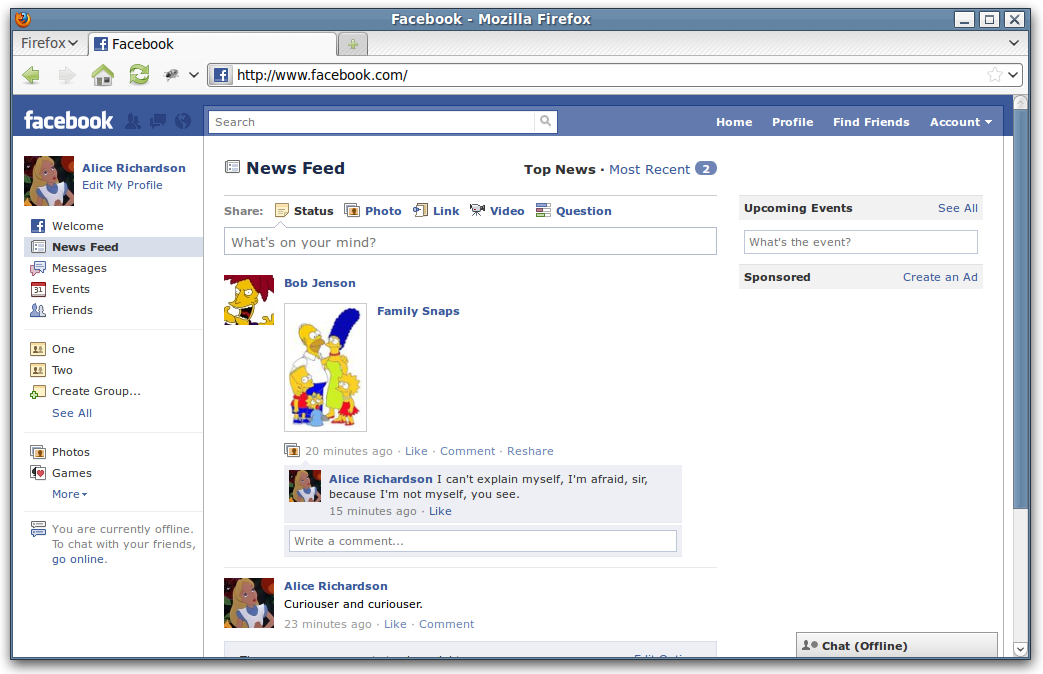
\includegraphics[width=12cm]{screens/facebook.png}
            \caption{News feed as presented on login.}
            \label{scn:fbook}
        \end{center}
    \end{figure}

\FloatBarrier
\subsection{Graph API}

Facebook does provide a JavaScript SDK for interfacing with the Facebook platform, however it is poorly documented and doesn't allow uploading images - since most JavaScript applications are designed to run inside the browser sandbox without local filesystem access. Instead, we may use the Facebook Graph API directly.

Objects can be read simply by making GET requests to \url{https://graph.facebook.com/ID} and parsing the return result as a JSON object. For none public objects we will also require an access token. Facebook uses the OAuth 2.0 protocol. An access token can be obtained by handling the page redirect \footnote{To ensure authentication can only occur in client side code the access token is passed in a URI fragment.} after the following GET request:

\FloatBarrier
    \begin{lstlisting}[label=code:auth,caption=Authentication GET request,float=h]
        https://www.facebook.com/dialog/oauth?
            client_id=APP_ID&
            redirect_uri=REDIRECT_URL&
            scope=SCOPE_VAR1,SCOPE_VAR2,SCOPE_VAR3&
            response_type=token
    \end{lstlisting}
\FloatBarrier

    
Content can also be published in a similar way. An example request might look like:

\FloatBarrier
    \begin{lstlisting}[label=code:pub,caption=Publishing POST request,float=h]
        https://graph.facebook.com/ID/feed?
            access_token=ACCESS_TOKEN&
            message=MESSAGE
    \end{lstlisting}
\FloatBarrier    

<--------------------------------------------------------------------->
<--------------------- Probably move this to Appendix ---------------->    

There are several caveats:

\begin{itemize}

    \item When publishing images, although the operation is supported, getting a correct handle to the image is difficult due to JavaScript's poor support for working with local files. The workaround requires creating an invisible form on the current page with a file input element and extracting the file handle from there.

    \item Images have to be published to an album. Facebook currently uses two types of album ID, one which appears within web pages and one which can be used for publishing through the Graph API. An additional API query is required before uploading to translate from one format to the other.
    
    \item It certain cases, though publishing through the Graph API is possible, it is more convenient to programatically manipulate form controls. An example is when submitting a comment and triggering the click handler for the submit button.
    
    \item Modifying the "About Me" section of a users profile is unsupported entirely. The workaround requires creating an invisible iframe on the current page and manipulating a form on the Facebook site within.

\end{itemize}

<--------------------------------------------------------------------->


    
\FloatBarrier
\section{Storing data in images}

As well as being one of the most frequently used types of content, images have been highlighted as a prime privacy concern on social networks \cite{fb-images}. None of the existing work supports image encryption, though flyByNight discusses it as a possible extension.

The main problem is that, regardless of the input format, Facebook encodes all uploaded images using lossy JPEG. \footnote{Even if a file is already in the output format the compression process is repeated and information is lost.} This means we require some form of JPEG-immune coding to store the binary output of encryption in an image, such that even after undergoing compression we can exactly recover the original bytes.

We being by describing Facebook's JPEG compression process and evaluating naive attempts at encoding data in images, before proposing two more advanced approaches.

\FloatBarrier
\subsection{JPEG compression process}

Information is lost at several stages:

\begin{enumerate}

    \item Colour images are subject to a lossy colour space transform from RGB to YCrCb.
    \item The chrominance components Cr and Cb are subsampled at a rate half that of the luminance channel.
    \item The discrete cosine transform is applied to each 8x8 block using finite arithmetic.
    \item DCT coefficients are quantised according to values in a quantisation matrix.
    
\end{enumerate}

Note that chrominance subsampling means that colour images only provide a 50\% increase in capacity over a grayscale image of the same resolution. For simplicity we will only consider grayscale images. This leaves quantisation as the principle step at which information loss occurs.

Table \ref{tab:quants} displays the quantisation matrix used for a grayscale JPEG image downloaded from Facebook. Using this and several other compression parameters our best guess is that Facebook is using the {\tt libjpeg} library for compression, with a quality factor setting of 85. \footnote{Based on the output of the JPEG Snoop application for Windows.}

\begin{table}[tb]
\begin{center}
    %\definecolor{lgray}{hsb}{0.1, 0, 0.9}
    %\rowcolors{3}{white}{lgray}
    \begin{tabular}{|+c |^c |^c |^c |^c |^c |^c |^c |}
    \hline
    \multicolumn{8}{|c|}{\bf Quantisation Matrix} \\ \hline
    \hline
    5 & 3 & 3 & 5 & 7 & 12 & 15 & 18 \\ \hline
    4 & 4 & 4 & 6 & 8 & 17 & 18 & 17 \\ \hline
    4 & 4 & 5 & 7 & 12 & 17 & 21 & 17 \\ \hline
    4 & 5 & 7 & 9 & 15 & 26 & 24 & 19 \\ \hline
    5 & 7 & 11 & 17 & 20 & 33 & 31 & 23 \\ \hline
    7 & 11 & 17 & 19 & 24 & 31 & 34 & 28 \\ \hline
    15 & 19 & 23 & 26 & 31 & 36 & 36 & 30 \\ \hline
    22 & 28 & 29 & 29 & 34 & 30 & 31 & 30 \\ \hline
\end{tabular}
\end{center}

\caption{Quantisation matrix used by Facebook for luminance channel.}
\label{tab:quants}

\end{table}


\subsection{Naive data insertion}

To motivate the need for a more complex scheme, we describe two naive methods of coding data in images.

One approach would be to encode directly into greyscale pixel values with enough redundancy to overcome the information lost during compression. Another approach might be to similarly encode data into DCT coefficients of an existing JPEG image, since through the process of decompression and re-compression only a small amount of information is lost. The main source of information loss for the second approach is from capping DCT coefficients that don't map back to greyscale values in the range 0-255.

\begin{figure}[tbph]
  \begin{center}
\begin{tikzpicture}
    \begin{axis}[grid=major,xlabel=JPEG Quality Factor,ylabel=BER (\%), xmin=80, xmax=90,
    height=8cm,width=10cm,legend style={legend pos=north east}]
    
    \addplot
        table[x=QF,y=rgb] {gfx/error_rate0.data};
    \addplot
        table[x=QF,y=dct] {gfx/error_rate0.data};
    \legend{Pixels,DCT}
    
    \end{axis}
\end{tikzpicture}
    \caption{Bit error rate for varying quality factors.}
    \label{graph:ber0}
  \end{center}
\end{figure}

Figure XX graphs the bit error rate for both methods over a range of quality factors, using {\tt libjpeg} for compression. For encoding in DCT coefficients a special bitmask, generated from the quantisation matrix, is used in an attempt to reduce the incidence of capping (see appendix XXX for details). Modeling the compression process as a binary symmetric channel, Figure XX graphs the theoretical per-image capacity of each method for lossless data transmission (details for this calculation are given in Evaluation section XXX).


\begin{figure}[tbph]
  \begin{center}
\begin{tikzpicture}
    \begin{axis}[grid=major,xlabel=JPEG Quality Factor,ylabel=Capacity (KiB/image), xmin=80, xmax=90,
    height=8cm,width=10cm,legend style={legend pos=north west}]
    
    \addplot
        table[x=QF,y=rgb2] {gfx/error_rate0.data};
    \addplot
        table[x=QF,y=dct2] {gfx/error_rate0.data};
    \legend{Pixels,DCT}
    
    \end{axis}
\end{tikzpicture}
    \caption{Per-image channel capacity (measured in KiB/image) for varying quality factors.}
    \label{graph:capacity0}
  \end{center}
\end{figure}

Given a recipient group size of 400 and ciphered session key size of 1024-bit (see section XXX), the transmission overhead required would be at least 50 KiB. This means neither of the naive approaches would be suitable, even given an error correction scheme which performs at or near the Shannon limit. 


\subsection{Advanced data insertion}

One initial optimisation for any coding scheme would be to map binary data to appropriate length gray codes to ensure that only single bit errors occur from erroneously outputting an adjacent codeword. In addition, we present two possible schemes, henceforth referred to as the HWT (Haar Wavelet Transform) method and the n-bit scaling method.

\begin{sdesc}

    \item[HWT method] \hfill \\ JPEG DCT compression selectively quantises perceptually redundant high frequency components. Wavelet transforms allow us to embed data in the low frequency sub-band of the carrier signal and can be performed reversibly (i.e. losslessly) by using an integer lifting scheme. Xu et al demonstrate that data encoded in low-frequency HWT approximation coefficients can survive JPEG decompression when combined with an error correction scheme \cite{haar}.
    
    \item[N-bit scaling method] \hfill \\ This method maps the n-bit input space on to the 8-bit pixel space by scaling the input such that 0 corresponds to 0, and $2^n - 1$ corresponds to 255. The inverse process amounts to outputting the interval the pixel value lies in. This method works on the assumption that large changes in pixel intensity are unlikely.

\end{sdesc}

Clearly both these schemes are sub-optimal and their exact properties (compression time and error rates) are unknown. We make it a requirement that the project should take a modular approach to conduit image implementations: firstly to ensure that both of the proposed schemes can be implemented simultaneously and their performances compared; secondly, to aid future development of a more optimal solution.



\FloatBarrier 
\section{Further security considerations}
\label{sec:security}

In order to meet the goal of privacy protection we must consider proper security engineering practices. A particular concern is that of introducing new vulnerabilities into the browser platform. We perform a threat analysis and describe issue relating to the underlying cryptographic scheme and management of private keys.

\FloatBarrier
\subsection{Threat analysis}
\label{ssec:threat}

Full details of the threat and risk analysis are included in appendix XXX. We take an attack-centric approach, defining risk as (Vulnerability x Threat x Impact) according the methodology described by \cite{XXX}. We identify several potential threats and possible security measures proportionate to the risk they pose:


\begin{sdesc} \addtolength{\itemsep}{-0.5\baselineskip}
    \item[Attack 1] Attacker breaks encryption scheme by brute force methods.
    \item[Measures] Ensure key sizes are appropriate given the type of attacker. See section XXX.
\end{sdesc}

\begin{sdesc} \addtolength{\itemsep}{-0.5\baselineskip}
    \item[Attack 2] Attacker gains access to user's computer by through the download and execution of a file.
    \item[Measures] Ensure only legitimate JPEG and public key files are downloaded. Public key files can be vetted on their character set and size, JPEG's by their extension.
\end{sdesc}

\begin{sdesc} \addtolength{\itemsep}{-0.5\baselineskip}
    \item[Attack 3] Attacker gains access to users computer by injecting code into eval() which runs outside the browser sandbox.
    \item[Measures] Wrap all calls to eval() with a SecureEval() function which sanitizes input and prevents malicious use. 
\end{sdesc}

\begin{sdesc} \addtolength{\itemsep}{-0.5\baselineskip}
    \item[Attack 4] Attacker gains access to Facebook account through browser code injection.
    \item[Measures] Sanitize all user inputs and ensure sanitisation can't be bypassed e.g. through UTF-8 decoder \cite{XXX}. Also sanitize output whenever inserting code into the DOM.
\end{sdesc}

\begin{sdesc}\addtolength{\itemsep}{-0.5\baselineskip}
    \item[Attack 5] Attacker carries out middle-person attack by intercepting and switching public keys.
    \item[Measures:] As stated in section \ref{sec:limit} protection from this type of attack is a non-goal. However, informing the user whenever public keys are updated removes a large amount of risk.
\end{sdesc}

\begin{sdesc} \addtolength{\itemsep}{-0.5\baselineskip}
    \item[Attack 6] Attacker causes DoS by creating a malicious object.
    \item[Measures] Since the decryption process is built to fail gracefully (see section XXX) this need not be a large problem even in the worse case, provided some simple run time checks are included.
\end{sdesc}


\FloatBarrier
\subsection{Underlying encryption schemes}

We use AES and RSA as both schemes are approved by NIST standards \cite{nist} and widely available via the Botan cryptography library. Ideally however, we would have liked to use a scheme based on elliptic curve cryptography since public key sizes are much smaller for the same amount of security than finite field or integer factorisation. This is important since the block size of the cipher depends on the public key, and this in turn determines the size of the session key once it has been encrypted. In our case, for example, a 256-bit AES session key requires 2048-bits of transmission overhead per recipient. Unfortunately ECC is less common in open libraries due to patent concerns \cite{XXX}.

Again, we make it a requirement that the project be modular enough to allow later use of a more suitable scheme.


\FloatBarrier
\subsection{Cryptographic keys}
\label{ssec:keys}

NIST(National Institute of Standard and Technology) provide recommendations on key size. Since 2010 NIST have recommended using at least 128-bits of security. This is equivalent to 3-TDEA (symmetric) or 2048-bit RSA (asymmetric). \cite{nist}

NIST also give recommendations for acceptable psuedo-random number generators and hash functions when generating keys, which we adhere to. {\tt /dev/random} is used as a source of entropy, an analysis of which is provided by http://www.pinkas.net/PAPERS/gpr06.pdf.
	
    

\FloatBarrier
\section{Requirements specification}

Based on the contents of this chapter we derive a set of concrete requirements.
        
\begin{desc}

    \item[Requirement 1] The extensions will be able to broadcast-encrypt, submit, retrieve and decipher the following objects:
    
    \begin{itemize}
        \item Status updates
        \item Wall posts
        \item Comments
        \item Messages
        \item Images
    \end{itemize}
    
    Specifically, key sizes will provide at least 128 bits of security according to the NIST standards described in section XXX.
    
    \item[Requirement 2] The size limits for encrypted text objects will be no smaller than the current limits Facebook imposes, given in section XXX).

    \item[Requirement 3] The size limit for encrypted images will be no less than 50 KiB. XXX JUSTIFY THIS XXX.

    \item[Requirement 4] To ensure the goal of scalability is met, all requirements will be met given recipient groups sizes up to 400, based on the discussion in section XXX.
    
    
    \item[Requirement 5] To ensure the goal of usability is met, response times will meet the criteria described by \url{http://www.useit.com/papers/responsetime.html}.


    \item[Requirement 6] Should try not to introduce any security holes. Up to a point, given scope of project. We have already declared a threat model and testing strategy etc.


    \item[Requirement 7] The number of newsfeed entries generated by encrypted submission will be no more than the number generated by normal content submission. This ensures that the effect on signal-to-noise ratio is kept to an absolute minimum - the only perceivable 'noise' is the encrypted content itself.
    

    \item[Requirement 8] There are uncertainties and/or trad-offs associated with certain approaches to encryption and encoding data in images (and to a lesser extent error correction). It is also clear that in some cases the optimal approach is well beyond the scope of this project. Therefore, we make it a requirement to adopt a modular structure that facilitates switching between differing schemes and permits future extension.
    
\end{desc}


   
\FloatBarrier 
\section{Development}
        
An agile development style was adopted based on \cite{XXX}. Uncertainties in the optimal approach or combination of approaches for encryption, image coding and error correction meant that being flexible and able to respond to changes was crucial. Delivering functional prototypes at various stage in the development life-cycle also fits with the project's modularity requirement. Since the bulk of the project concerns encapsulating data in some layer of encoding the natural approach was to build successive prototypes, each implementing a new layer.

\subsection{Development environment}

Git was used for revision control and backup. The working repository is stored on a laptop and pushed twice-daily to a remote repository hosted by ProjectLocker.

Komodo edit was used as a development IDE, as recommended by Mozilla. C++ coding style followed the guidelines detailed here \cite{code-style} and documentation was generated automatically using Doxygen.

Firefox 4.0 pre-beta was obtained through APT by adding the Mozilla Daily Build Team PPA. The build process consists of compiling and linking the C++ shared library, then packaging this (together with the rest of the extension code) and automatically installing to a number of Firefox development profiles.        

GNU Octave (a free MATLAB-like application) was also used for provisional evaluation and to generate some of the results in this section.



\FloatBarrier
\section{Testing plan}

General testing followed the agile testing principles of "test driven" development over "test last". The feedback loop between testing and implementation was kept as short as possible, to maintain flexibility over the exact approach.


\subsection{Security testing}

Special attention was made to security relevant testing such as input sanitisation and proper functioning of the UTF-8 decoder. Boundary-value analysis was used to generate sets of test scripts (included in appendix XXX).


\subsection{Usability testing}

To help ensure the goal of usability was met, usability testing in the form of cognitive walkthroughs were performed. During development many passes of the walkthroughs were performed and alterations made, until a credible success story could be constructed for each task. Excerpts from final success stories are presented in evaluation chapter XXX.


\subsection{Testing framework}

In order to expedite testing often the Facebook image compression process was simulated locally. We used libjpeg at quality factor 85 since this most closely matches the compression signature of Facebook images.

The C++ module was developed and unit tested offline independently. Testing codes was built into extraneous library functions and {\tt gprof } was used for profiling and debugging.

Once the JavaScript module was built integration testing was performed. ChromeBug, FireBug and FireUnit were used for testing, profiling and debugging.

